\section{Simulação de Rede de Comunicação Subaquática}
\label{sec:simulacao-rede-comunicacao-subaquatica}

\subsection{Desafios da Comunicação Subaquática}
\label{subsec:desafios-da-comunicacao-subaquatica}

A utilização de sistemas de comunicação subaquática em veículos autônomos é uma tarefa desafiadora. Nos últimos anos, no entanto, pesquisadores estão encontrando soluções para implementar esses sistemas através de rede sem fio.

Nesse cenário, estão sendo desenvolvidas tecnologias voltadas a redes de sensores subaquáticos (UWSNs, do inglês \textit{underwater wireless sensor networks}), onde estas são compostas por nós que recebem, coletam e transmitem informações para os \textit{gateways} de superfície \cite{godi2021survey}. Dentre diversas opções, destaca-se três formas principais para se comunicar através da água: sensores acústicos, radiofrequência e dispositivos ópticos.

Os sistemas ópticos e de radiofrequência são limitados pelo alto nível de absorção na água. Já os sistemas de comunicação acústica são a forma preferencial para comunicações subaquáticas sem fio, pois apresentam baixa atenuação na água \cite{vieira2010redes}. 

Na superfície existem meios de comunicação utilizando ondas eletromagnéticas, como GPRS e Iridium, que podem ser usados para transferência de pequenas quantidades de dados e principalmente comandos, e o Wi-Fi, para curto alcance. Alguns veículos subaquáticos utilizam tecnologias como comunicação de radiofrequência de 900 MHz, que corresponde a um \textit{trade-off} entre alcance e taxas de transferência.


\subsection{Arquiteturas de Comunicação Subaquática}
\label{subsec:arquiteturas-de-comunicacao-subaquatica}

Para a comunicação com a superfície, a disponibilização dos sensores no ambiente hídrico depende da topologia da rede adotada, que leva em conta consumo de energia, confiabilidade e capacidade da rede, bem como objetivo da missão. As arquiteturas de comunicação subaquática podem ser classificadas em três tipos: bidimensional estático, tridimensional estático e tridimensional com veículos autônomos subaquáticos (AUV, do inglês \textit{autonomous underwater vehicles}) \cite{akyildiz2005underwater}.

Na arquitetura de comunicação 2D estática, conforme mostra a Figura \ref{fig:arquitetura-rede-2d}, todos os nós de sensores são ancorados no fundo do oceano e a comunicação desses nós de sensores subaquáticos ocorre por meio de interligação de um ou mais \textit{underwater sinks} (uw-sinks), através de um \textit{link} acústico de comunicação. 

\begin{figure}[h]
	\centering
	\caption[Arquitetura para redes de sensores subaquáticos 2D]{Arquitetura para redes de sensores subaquáticos 2D}
	\label{fig:arquitetura-rede-2d}
	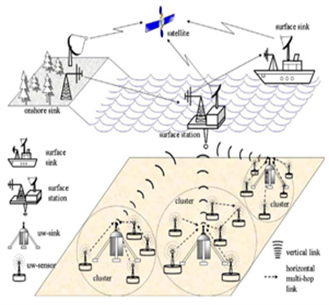
\includegraphics[width=0.5\linewidth]{images/arquitetura-rede-2d}\\
	\footnotesize Fonte: \cite{akyildiz2005underwater}
\end{figure}

No modelo 3D estático, conforme mostra a Figura \ref{fig:arquitetura-rede-3d}, os nós dos sensores são colocados em profundidades distintas (inclusive flutuantes) para observar determinado fenômeno. Já a arquitetura 3D com AUV consiste em nós de sensores estáticos colocados no fundo do oceano, nós de sensores em diferentes profundidades e sensores móveis.

\begin{figure}[h]
	\centering
	\caption[Arquitetura para redes de sensores subaquáticos 3D]{Arquitetura para redes de sensores subaquáticos 3D}
	\label{fig:arquitetura-rede-3d}
	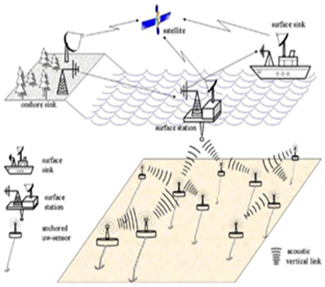
\includegraphics[width=0.5\linewidth]{images/arquitetura-rede-3d}\\
	\footnotesize Fonte: \cite{akyildiz2005underwater}
\end{figure}

Em uma UWSN implantada em uma área para ser monitorada, os sensores subaquáticos são conectadas digitalmente a uma estação remota através da internet, as informações coletadas pelos nódulos dos sensores são transmitidas para os \textit{gateways} de superfície por meio da comunicação acústica, e as informações são retransmitidas para o centro de monitoramento remoto. Os \textit{gateways} de superfície são equipados com \textit{modens} acústicos e outras tecnologias com a radiofrequência ou sensores óticos (veja Figura \ref{fig:arquitetura-comunicacao}).

\begin{figure}[h]
	\centering
	\caption[Arquitetura de Comunicação Subaquática]{Arquitetura de Comunicação Subaquática}
	\label{fig:arquitetura-comunicacao}
	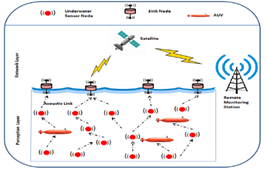
\includegraphics[width=0.5\linewidth]{images/arquitetura-comunicacao}\\
	\footnotesize Fonte: \cite{godi2021survey}
\end{figure}

\subsection{Características da Comunicação Acústica}
\label{subsec:caracteristicas-da-comunicacao-acustica}

\subsubsection*{Camada física}

Camada física em termos de redes, é a primeira camada que se refere aos meios de conexão através dos quais irão trafegar os dados. É nela que são especificadas as funções e protocolos necessários para a transmissão dos bits entre dois dispositivos, tais como interfaces seriais, ou cabos coaxiais \cite{Wikipedia}.

No caso da comunicação acústica, o meio de físico de transmissão é o aquático, e este influencia diretamente nas camadas de protocolo, desde camada física até a camada de aplicação.

Sendo assim, em relação ao meio físico terrestre, existe uma série de restrições no meio aquático, o que caracteriza unicamente os sensores no ambiente hídricos. Desse modo, apesar da comunicação acústica ser melhor opção entre a ótica e a radiofrequência, a tecnologia caracteriza-se por uma série de desafios por causa da alta latência para a propagação sinal, a largura de banda é atenuada, depende da frequência e do alcance, possui uma alta atenuação, e ainda ocorre uma elevada taxa de erros na transmissão dos bits devido a problemas como desvanecimento multi-caminho (do inglês \textit{multipath fading}). Ao mesmo tempo, que os dispositivos se movem na água devido as correntes marítimas \cite{vieira2010redes}.

\subsubsection*{Utilização do canal}

A eficiência da utilização do canal acústico é dada de acordo com o tamanho do pacote, ou seja, quanto maior o tamanho do pacote, maior a probabilidade desse ser recebido com erro. No entanto, devido ao envio de erros aumenta-se a retransmissão de dados e diminui-se a utilização do canal, chegando-se a um ponto ótimo.

\subsubsection*{Camada de enlace}

A camada de enlace é responsável por corrigir os erros que podem ocorrer na camada física. É composta pelos protocolos MAC (do inglês \textit{Media Access Control}), que melhoram a eficiência transmissão e provêm acessos mais equitativos à rede (\textit{fairness}), além de controlar o acesso ao meio comum compartilhado por diversos usuários.
 
\underline{Protocolos MAC Baseados em Partição}

Dentre diversos protocolos baseados em partição, destacam-se \cite{vieira2010redes}:

\begin{itemize}
	\item FDMA: Acesso múltiplo dividido pela frequência (do inglês \textit{frequency division multiple access});
	\begin{itemize}
		\item Divide a frequência de banda disponível em múltiplas sub bandas e assinala cada sub banda a um nó individual;
		\item Vantagem: algoritmo simples e eficiente em um pequeno número de nós;
		\item Desvantagens: não dá para usar na rede subaquática por causa da frequência de banda.
	\end{itemize}
	\item TDMA: Acesso múltiplo dividido pelo tempo (do inglês \textit{time division multiple access});
	\begin{itemize}
		\item Divide em múltiplos períodos, em que cada período é unicamente assinalado a um nó individual;
		\item Vantagem: utiliza \textit{buffer} em vez de período;
		\item Desvantagem: requer sincronização de tempo precisa entres os nós.
	\end{itemize}
	\item CDMA: Acesso múltiplo dividido codificado (do inglês \textit{code division multiple access}).
	\begin{itemize}
		\item Toda a frequência de banda é operada de forma concorrente por múltiplos nós. Para isso, o acesso ao canal é baseado em um código único que é usado para espalhamento;
		\item Vantagem: Apresenta bom desempenho em águas rasas;
		\item Desvantagem: é vulnerável ao problema perto–longe (também conhecido como \textit{near-far problem}).
	\end{itemize}
\end{itemize}

\underline{Protocolos Baseados em Acesso Aleatório}

Neste protocolo, os recursos limitados do canal não são divididos, e o meio é acessado pelos nós através do princípio de contenção \cite{vieira2010redes}.

\begin{itemize}
	\item O protocolo ALOHA original é baseado em um acesso aleatório puro ao meio. A vazão máxima alcançável dele é 18\%, devido a retransmissões e contenções.
	\item O protocolo Aloha-CA (do inglês \textbf{Aloha with Collision Avoidance}) é baseado no ALOHA original. Nele, tenta-se evitar colisões e se obtém desempenho de vazão por meio da redução do tamanho do cabeçalho da mensagens transmitidas.
	\item O protocolo Aloha-AN (do inglês \textit{Aloha with Advance Notification}) é baseado no ALOHA-CA e tem a mesma proposta. A diferença é que transmite no pacote a notificação avançada (NTF) em cada nó, o que dá ao mesmo um subconjunto maior do estado da rede, permitindo tomar-se uma decisão melhor para evitar-se colisões.
	\item O protocolo CSMA (do inglês \textit{Carrier Sense Multiple Access}) tenta evitar colisões consultando ou escutando os nós vizinho antes transmitir a mensagem. Nesta abordagem, as colisões são tratadas pelo transmissor. Existem diversas variantes dos métodos na literatura que incluem controles como RTS (do inglês \textit{request-to-send}) e CTS (\textit{do inglês clear-to-send}).
\end{itemize}

\underline{Protocolos Baseados em Reserva e Escalonamento}

Nesse tipo de protocolo utiliza-se escalonamento determinístico ou pré-definido para que os nós acessem o canal, o que aumenta a utilização do mesmo e diminui as colisões, sem ter a divisão de recursos. Todavia não é possível dinamizar a rede como juntar um nó à rede, retirar, falhar ou mover. Dentre as variações destaca-se o Protocolo MAC Baseado em Reserva (R-MAC) que é um tipo de CSMA baseado em escalonamento. Com ele é possível alcançar eficiência de energia usando escuta periódica e modos de ``dormir'' para reduzir o gasto de energia em estados ociosos.

\subsubsection*{Roteamento}

Os protocolos de roteamento móvel criados para o meio terrestre são classificados como proativos, reativos ou geográficos. Estes protocolos não são adequados para as redes subaquáticas devido à imprecisão neste ambiente e a necessidade de estabelecer um caminho de rota (no caso do proativo). Além disso, apresentam alta latência ocasionada pelo meio, o que aumenta ainda mais a lentidão da propagação de sinal em redes acústicas (no reativo). Por fim, possuem necessidade de adaptação ou uso consorciado para o ambiente subaquático, como é o caso do GPS (do inglês \textit{Global Positioning System}) e outras tecnologias similares do tipo geográfico. 

De outro modo, novas tecnologias apresentam protocolos para redes subaquáticas baseados em pressão, onde o roteamento é feito através do encaminhamento de pacotes tendo como base a medida do nível de pressão (ou profundidade) em cada nó.


\subsection{Simulação da Comunicação}
\label{subsec:simulacao-da-comunicacao}

É extremamente caro e complexo implementar uma estrutura completa de rede subaquática com \textit{links} de dados para coletar e transmitir informações de uma coluna de água, composta por nós de sensores, \textit{gateways} na superfície e AUVs \cite{godi2021survey}. Os dispositivos custam caros por demandarem baias de proteção, são propensos a falhas por causa da corrosão e incrustações, as baterias limitadas não podem ser recarregadas com energia solar e a manutenção é complicada por estarem submersos \cite{akyildiz2005underwater, shantaram2005challenges}

Além do mais, é difícil validar os protocolos ou algoritmos usados na rede UWSN por meio de testes, que podem não ser adequado para todos os tipos de aplicações \cite{das2016simulation}.  

Diante do exposto, a existência de um ambiente de simulação que replicasse o cenário subaquático real, permitiria ao engenheiro ou pesquisador estudar os comportamentos com base nas características físicas, por meio dos testes de seus modelos em paralelo com a implementação em tempo real.

Assim, com base no projeto conceitual -- mostrado na Figura \ref{fig:conceito-final} -- elaborado após conclusão da matriz morfológica, foi proposta a arquitetura da rede de comunicação baseado no modelo 3D com AUV, onde serão dispostos aleatoriamente diversos modens acústicos que farão a transmissão de informação entre o BROV, a boia e objeto a ser capturado (representado pela moeda). Já o tráfego de dados responsável pela localização do AUV e do objeto a ser capturado será feito pela rede entre estes e o sensor de SBL.

\begin{figure}[h]
	\centering
	\caption[Projeto Conceitual]{Projeto Conceitual}
	\label{fig:conceito-final}
	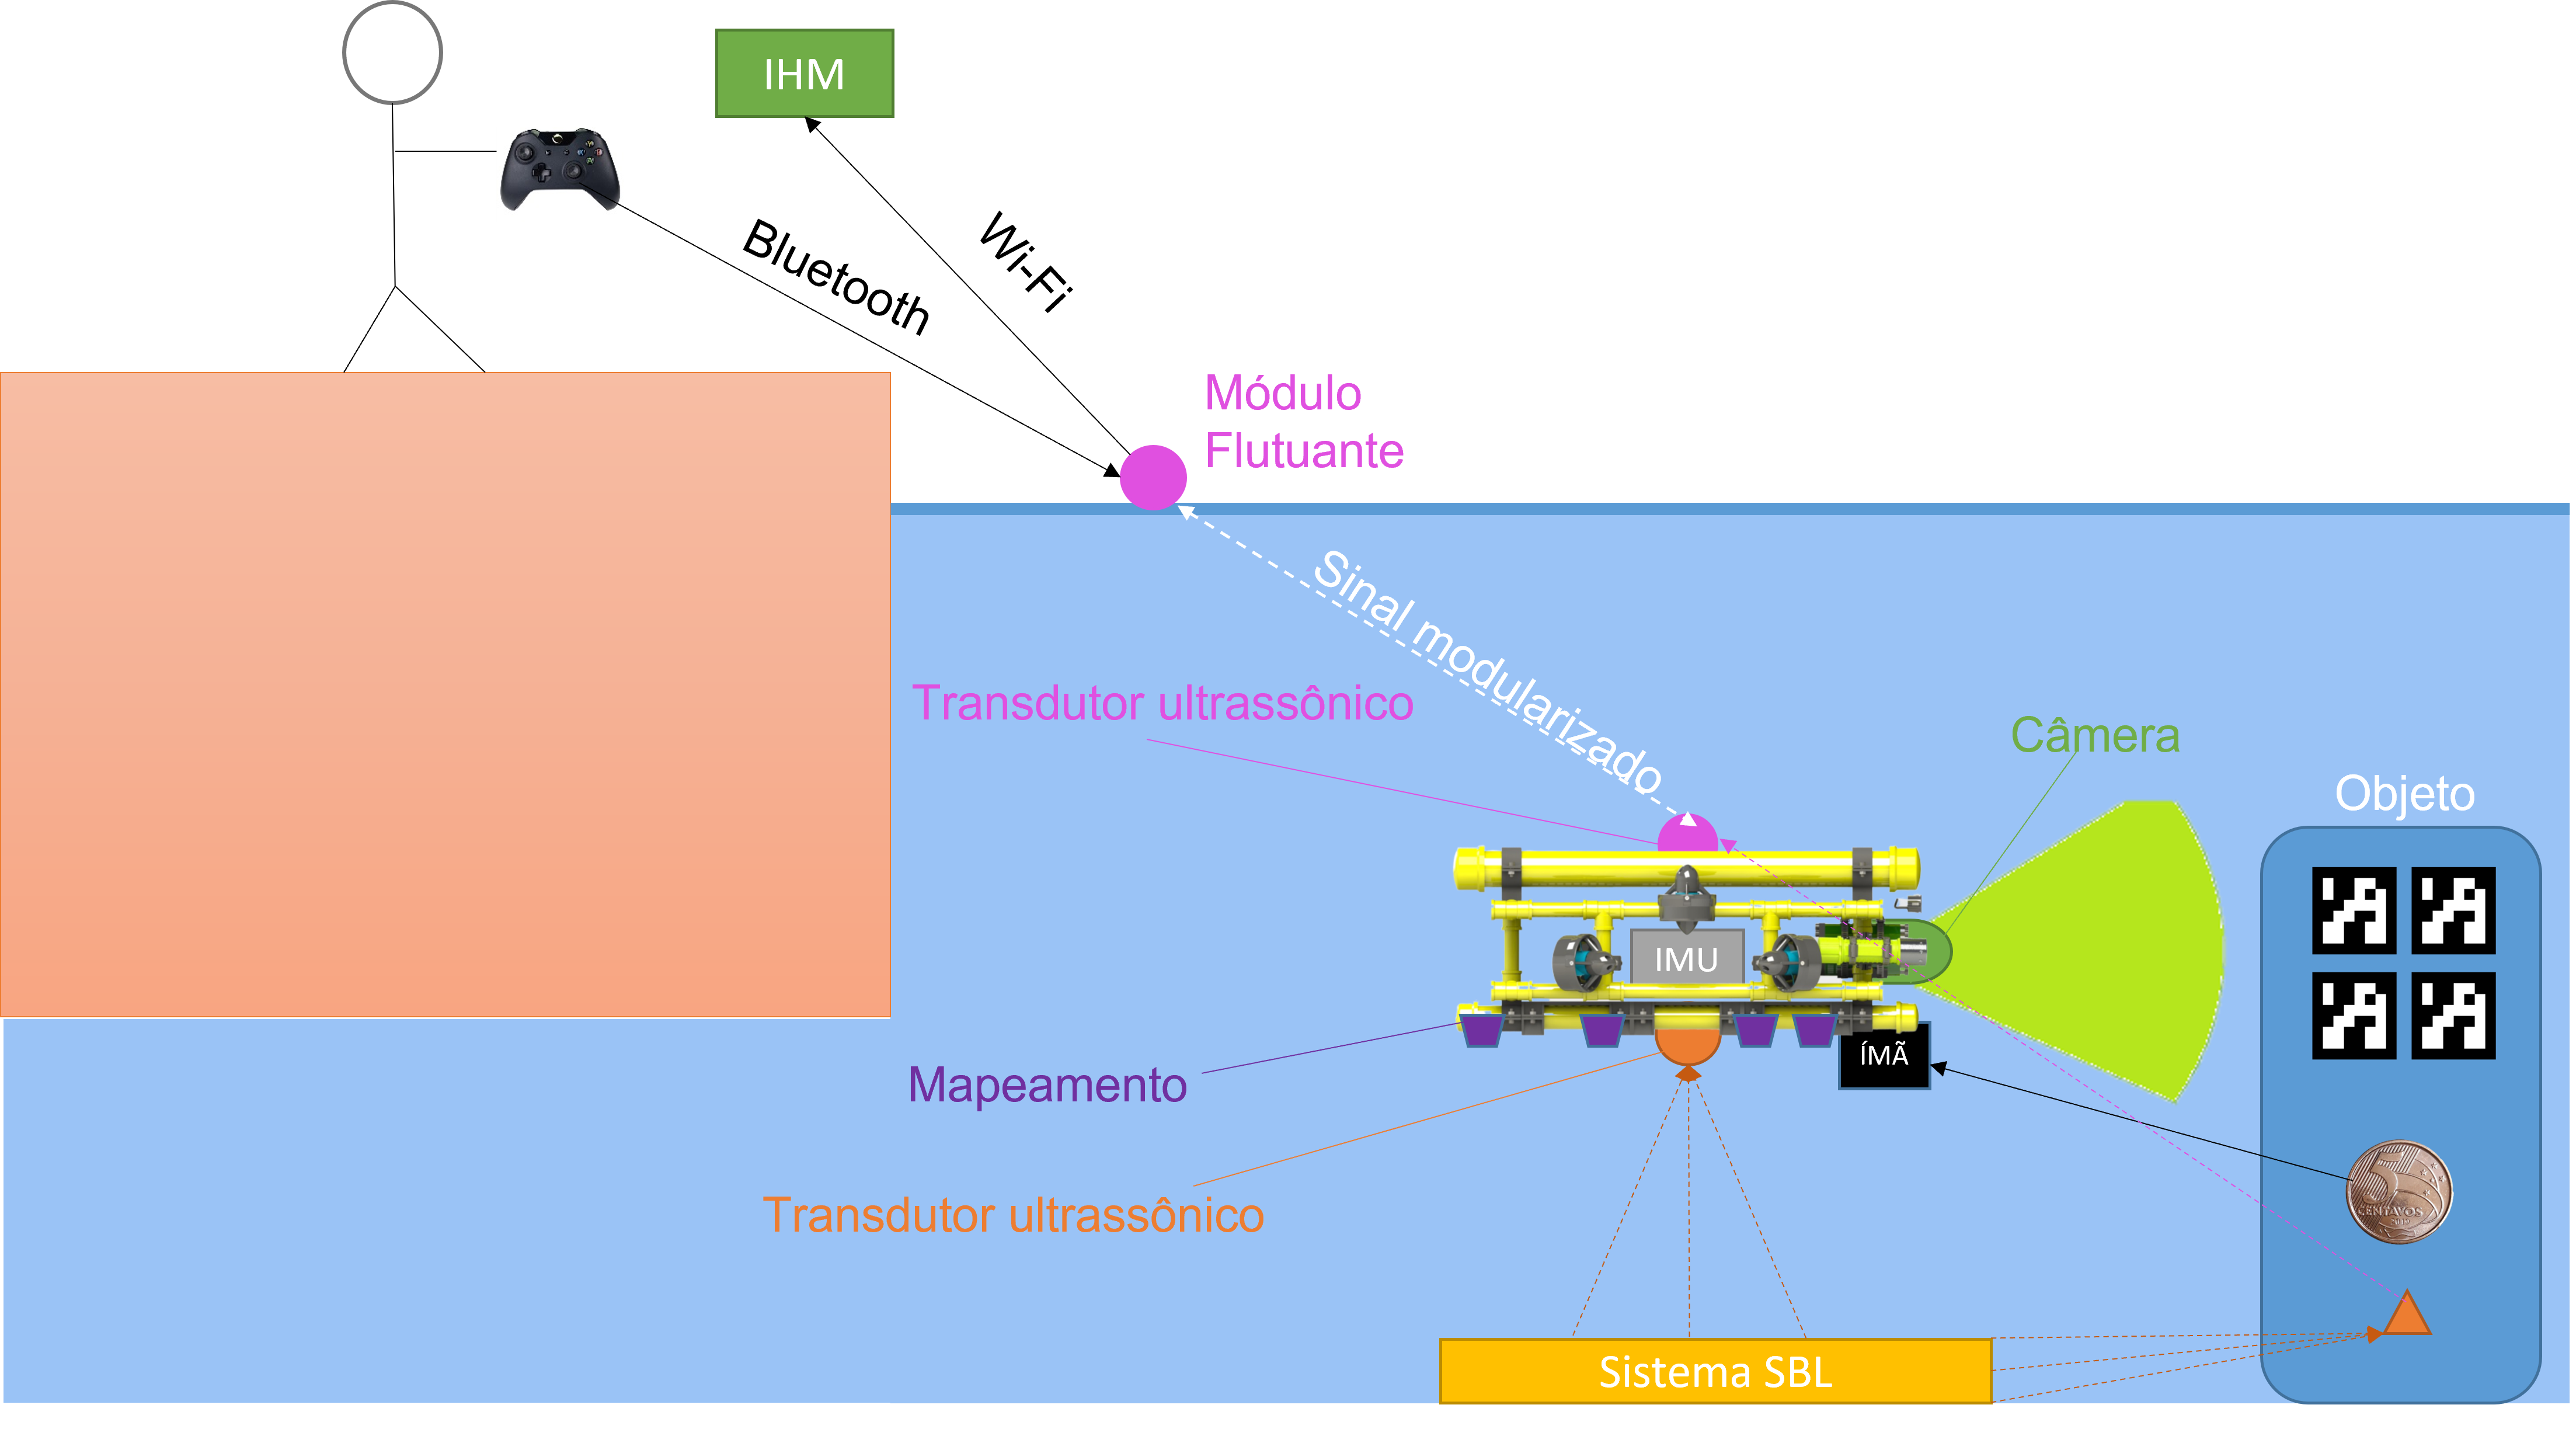
\includegraphics[width=0.8\linewidth]{images/conceito-final}\\
	\footnotesize Fonte: Autores
\end{figure}

Para simular a comunicação serão utilizados as bibliotecas para simulação escritas em Python que objetivam testar algoritmos da rede acústica NM3, desenvolvida no laboratórios USMART (do inglês \textit{Smart Dust for large scale underwater wireless sensing}) \cite{8248761} e o AUVNetSim: A Simulator for Underwater Acoustic Networks  \cite{montana2008auvnetsim}. 

O NM3 é uma alusão aos modens acústicos subaquáticos NM3 também conhecidos como “NanoModem”. A biblioteca possui uma coleção de utilitários e de drivers escritos para facilitar o trabalho com estes dispositivos. Permite também controlar os pacotes da transmissão de mensagens por meio de protocolos, gerar \textit{logs}, controlar e simulador modens acústicos virtuais \cite{SHERLOCK2019}.

O AUVNetSim contém um pacote com uma grande variedade parâmetros, mostrados na Tabela \ref{tab:parametros}, e protocolos para redes acústicas subaquáticas que podem ser selecionados ou modificados para implementar novos protocolos aproveitando a estrutura existente.

\begin{table}[h]
	\centering
	\caption[Parâmetros AUVNetSim que devem ser especificados no arquivo de configuração]{Parâmetros AUVNetSim que devem ser especificados no arquivo de configuração}
	\label{tab:parametros}
	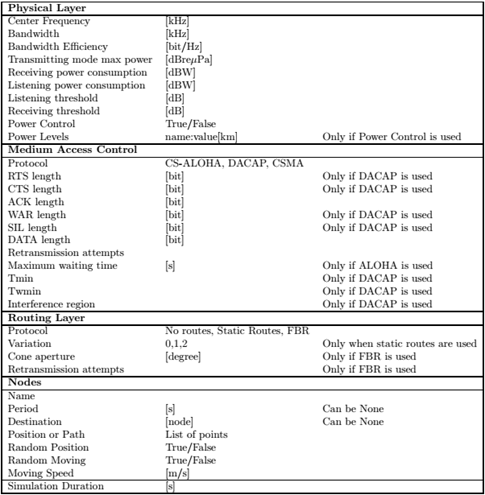
\includegraphics[width=0.8\linewidth]{images/parametros}\\
	\footnotesize Fonte: \cite{montana2008auvnetsim}
\end{table}

Além disso, na simulação de cada nó acústico a comunicação é realizada por troca de mensagens curtas entre as camadas que podem ser configuradas na seguinte ordem: física, MAC, roteamento e aplicação. Essa configuração está apresentada na Figura \ref{fig:auvnetsim}

\begin{figure}[h]
	\centering
	\caption[Estrutura de programação de um nó acústico AUVNetSim]{Estrutura de programação de um nó acústico AUVNetSim}
	\label{fig:auvnetsim}
	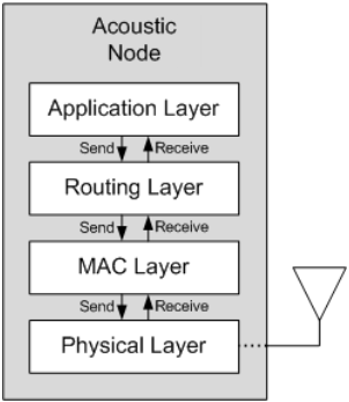
\includegraphics[width=0.3\linewidth]{images/auvnetsim}\\
	\footnotesize Fonte: \cite{montana2008auvnetsim}
\end{figure}

Apesar de existirem outras propostas de ferramentas disponíveis no mercado com mesma característica e até melhores que o AUVNetSim ou NM3, como Network Simulator (NS-3), SUNSET ou Aqua-Sim que permitem, além da emulação, testes em tempo real \cite{godi2021survey}. As bibliotecas foram selecionadas por serem de código aberto, e mesmo que ainda não testadas a fundo, possuem manual de utilização \cite{montana2008auvnetsim} e Wiki \cite{SHERLOCK2019} que é de fácil integração e manutenção. Além disso, os pré-requisitos não exigem recursos computacionais muito pesados para a sua utilização.

Assim, a adoção do AUVNetSim tem como objetivo integrá-la com o ROS (\textit{Robot Operating System}), com a finalidade de simular a comunicação entre os dispositivos em uma topologia de rede (em vermelho) com a arquitetura conforme proposto na Figura \ref{fig:arquitetura-comunicacao-brov}, e o NM3 para a comunicação da trilateração do SBL(em preto).

\begin{figure}[h]
	\centering
	\caption[Arquitetura de Comunicação do BROV]{Arquitetura de Comunicação do BROV}
	\label{fig:arquitetura-comunicacao-brov}
	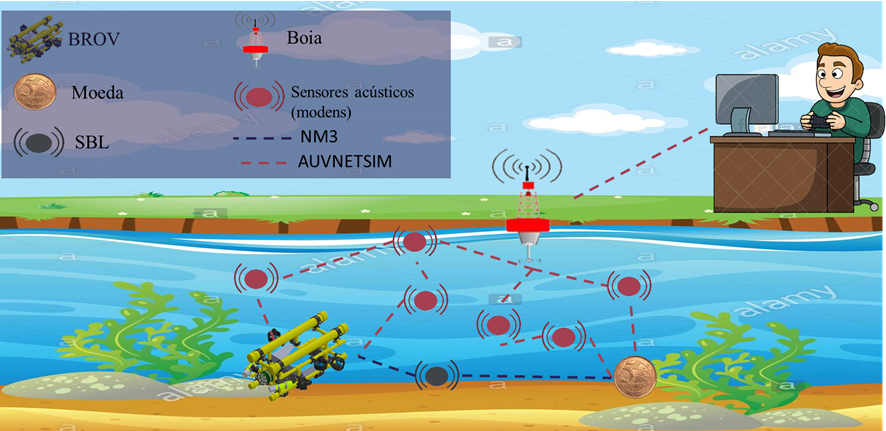
\includegraphics[width=1\linewidth]{images/arquitetura-comunicacao-brov}\\
	\footnotesize Fonte: Autores
\end{figure}

